\documentclass[a4paper]{article}
\usepackage[pdftex]{graphicx}
\usepackage[utf8]{inputenc}
\usepackage{enumerate}
\usepackage{amssymb}
\usepackage{icomma}
\usepackage{siunitx}
\sisetup{locale=DE} 
\usepackage{tikz}
\usepackage{href-ul}
\hypersetup{
	colorlinks=true,
	linkcolor=blue,
	urlcolor=blue}
\usepackage{geometry}
\geometry{a4paper, top=15mm, left=15mm, right=15mm, bottom=15mm,
	headsep=10mm, footskip=12mm}

\begin{document}
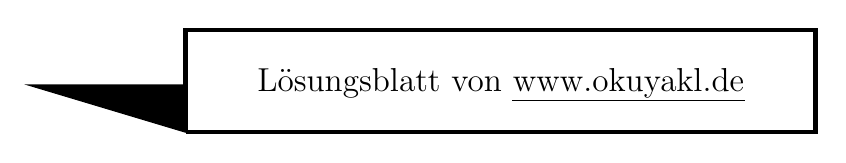
\begin{tikzpicture}(10,3)
	\draw[ultra thick](2,0) --(10,0) -- (10,1.3) --(2,1.3) -- (2,0);
	\draw[fill=black](2,0)-- (0,.6) -- (2,.6) -- (2,0);
	\node at (6,.6) {\large Lösungsblatt von \href{https://www.okuyakl.de}{www.okuyakl.de}};
\end{tikzpicture}
\vspace{0.5 cm}


\noindent{\bf Aufgabe 1. a)}\\
$$V= \SI{8,0}{\centi{\meter^3}}$$
\vspace{0.5 cm}

\noindent{\bf Aufgabe 1. b)}\\
$$ F_1 = m\cdot g = \varrho_{Cu}\cdot V \cdot g = \SI{0,70}{\newton} $$
\vspace{0.5 cm}

\noindent{\bf Aufgabe 1. c)}\\
$$ F_2 = \varrho_{Cu}\cdot V \cdot g - \varrho_{H_2O}\cdot V \cdot g = \SI{0,62}{\newton} $$
\vspace{0.5 cm}

\noindent{\bf Aufgabe 1. d)}\\
Sie zeigt zusätzlich das Gewicht der verdrängten Flüssigkeit an: Insgesamt $\SI{508}{\gram}$. Der Würfel hängt nach wie vor am Kraftmesser.
\vspace{0.5 cm}

\noindent{\bf Aufgabe 2. a)}\\
Der Pokal muss homogen sein, d.h. er darf z.B. keinen Fuß aus Stein o. ä. haben.\\
Der Messzylinder muss groß genug sein, damit der Pokal auch ganz hineinpasst und untergetaucht werden kann.\\
Der Silberbrocken muss groß genug sein, damit sein Volumen und sein Gewicht gut bestimmt werden kann.
\vspace{0.5 cm}
 
\noindent{\bf Aufgabe 2. b)}\\
\begin{itemize}
 \item Der Silberbrocken und der Pokal wird mit der Waage gewogen und das jeweilige Gewicht $m_s, \quad m_p$ notiert.
\item Der Messzylinder wird bis zu einer bestimmten Marke mit Wasser gefüllt.
\item Wir tauchen den Pokal in den Messzylinder vollständig ein und notieren den Anstieg des Füllstandes. $V_p$
\item Wir nehmen den Pokal wieder heraus, kontrollieren den Füllstand, und tauchen den echten Silberbrocken hinein. Wir notieren $V_s$.
\item Wir vergleichen: $$ {m_s \over V_s} \stackrel{?}{=} \quad {m_p \over V_p}  $$ Ist die Dichte gleich, dann handelt es sich beim Pokal um echtes Silber.
\end{itemize}
 
\vspace{0.5 cm}

\noindent{\bf Aufgabe 3. a)}\\
Die Differenz der Dichten ist:
$$\Delta\varrho={1\over 4}\cdot \SI{1,3}{\kilogram\over{\meter^3}}= \SI{0,33}{\kilogram\over{\meter^3}} $$ 
Die Nutzlast ist dann:
$$m=\Delta\varrho\cdot V = \SI{0,325}{\kilogram\over{\meter^3}} \cdot \SI{5000}{{\meter^3}}=\SI{1625}{\kilogram}\approx\SI{1,6}{\tonne}$$
\vspace{0.5 cm}

\noindent{\bf Aufgabe 3. b)}\\
Die Differenz der Dichten ist:
$$\Delta\varrho= \SI{1,3}{\kilogram\over{\meter^3}}-\SI{0,178}{\kilogram\over{\meter^3}} = \SI{1,1}{\kilogram\over{\meter^3}} $$ 
Das Volumen ist dann:
$$ V= {m \over \Delta\varrho}={\SI{1625}{\kilogram}\over \SI{1,122}{\kilogram\over{\meter^3}}}=\SI{1448}{{\meter^3}}\approx\SI{1,4e3}{{\meter^3}}$$
\vspace{0.5 cm}

\noindent{\bf Aufgabe 4.}\\
Die Dichte des Steins beträgt ${9\over 10}$ der Dichte der Flüssigkeit, also 
$$\varrho_{Stein}=0,9\cdot \SI{3,1}{\gram\over\centi{\meter^3}}=\SI{2,8}{\gram\over\centi{\meter^3}}$$
Das Volumen des Steins ist somit:
$$V_{Stein}={m \over \varrho_{Stein}}={\SI{80}{\gram}\over \SI{2,79}{\gram\over\centi{\meter^3}}}=\SI{28,7}{\centi{\meter^3}}\approx\SI{29}{\centi{\meter^3}}$$
\vspace{0.5 cm}

\noindent{\bf Aufgabe 5.}\\
Die Formel für den Schweredruck ist: 
$$p=g\cdot \varrho \cdot h =\SI{9,81}{\meter\over {\second^2}} \cdot \SI{1000}{\kilogram\over{\meter^3}}\cdot h = \SI{47}{\kilo\pascal}$$
\vspace{0.5 cm}

\noindent{\bf Aufgabe 6.}\\
\renewcommand{\arraystretch}{2}
\begin{tabular}{|p{1,2 cm}|p{1,7 cm}|p{1,7 cm}|p{1,7 cm}|p{1,7 cm}|p{1,7 cm}|p{1,7 cm}|p{1,7 cm}|}
	\hline
	& Nicht\-schwimmer\-becken & Sprung\-becken & Nordsee & Bodensee & Baikalsee & Atlantik & Mari\-anen\-graben \\
	\hline
	Tiefe h  &$\SI{1,20}{\meter}$ &$\SI{4,8}{\meter}$ &$\SI{50}{\meter}$ &$\SI{250}{\meter}$ &$\SI{1642}{\meter}$ &$\SI{3500}{\meter}$ &$\SI{11}{\kilo\meter}$ \\
	\hline
	Druck &$\SI{12}{\kilo\pascal}$ &$\SI{48}{\kilo\pascal}$ &$\SI{0,5}{\mega\pascal}$ &$\SI{2,5}{\mega\pascal}$ & $\SI{16}{\mega\pascal}$ &$\SI{35}{\mega\pascal}$ & $\SI{110}{\mega\pascal}$\\
	\hline
\end{tabular}

\begin{center}
	\includegraphics[width=7 cm]{../../viecher/endcomic.pdf}
	
	Hier geht es zurück zum \href{https://www.okuyakl.de/phys/p9achL078/aa078.pdf}{Aufgabenblatt}
\end{center}

\end{document}

